% !TeX root = ../main-english.tex
% !TeX spellcheck = en-US
% !TeX encoding = utf8
% -*- coding:utf-8 mod:LaTeX -*-

%This smart spell only works if no changes have been made to the chapter
%using the options proposed in preambel/chapterheads.tex.
\setchapterpreamble[u]{%
	\dictum[Albert Einstein]{We cannot solve our problems with the same level of thinking that created them}
}
\chapter{Introduction}
\label{chap:k1}

Look mom, some text!

\section{Brain state spaces}
This is an introduction into brain states and functional alignment
\pagebreak

\section{Magnetoencephalograpy (MEG)}
This is an introduction into \gls{meg} data
\pagebreak

\section{Research data management for computational modeling}
%This is an introduction on the importance of research data management for reproducible science

Research data encompasses everything that is produced in the life span of a research project.
This could include raw data acquisitions, preprocessed or otherwise standardized datasets, software, analysis scripts, results, compiled reports or articles, figures, tables, and many other final or intermediate outcomes of a research process.
To disambiguate ``research data'' from the smaller-scoped meaning that terms such as ``data'' or ``dataset'' carry in colloquial language (for example, the outcome of a data acquisition in an experiment), it is also referred to in the literature as ``research objects``, and, in case it exists in purely electronic form, as ``digital research objects''. (CITATION NEEDED)
\gls{rdm} describes the handling of these research objects through their entire life cycle: from curation, use, publication and sharing, archiving to re-use or destruction.
Typically, research objects have a much longer life span than the project that creates them.
Research data management ensures that research objects are preserved to act as an evidence base for findings and as a resource for further reuse.
As such, \gls{rdm} is a foundational element within good scientific practice, and, as I will lay out in this section and in upcoming chapters, an important prerequisite for computational modeling.


\subsection{The FAIR guiding principles for scientific data management and stewardship}

Since their publication, the so-called \glsunset{FAIR}\gls{FAIR} principles \citep{wilkinson2016fair} have become guidelines for \gls{rdm} efforts for digital research objects.
They describe four measurable properties of research data that -- the better they are fulfilled -- serve the ultimate goal to improve the discoverability and reusability of data by machines and humans alike \citep{wilkinson2016fair}.
The \gls{FAIR}ness of data can be improved on each of the four related but separable major characteristics that are behind the \gls{FAIR} acronym (taken verbatim from \citet{wilkinson2016fair}):

\begin{itemize}
	\item \textbf{F}indable: To be Findable, (meta)data  are assigned a globally unique and persistent identifier (F1); data are described with rich metadata (F2); metadata clearly and explicitly include the identifier of the data it describes (F3);  (meta)data are registered or indexed in a searchable resource (F4)
	\item \textbf{A}ccessible: To be Accessible, (meta)data are retrievable by their identifier using a standardized communications protocol (A1); the protocol is open, free, and universally implementable (A1.1); the protocol allows for an authentication and authorization procedure, where necessary (A1.2);  metadata are accessible, even when the data are no longer available (A2)
	\item \textbf{I}nteroperable:  To be Interoperable, (meta)data use a formal, accessible, shared, and broadly applicable language for knowledge representation (I1); (meta)data use vocabularies that follow FAIR principles (I2); (meta)data include qualified references to other (meta)data (I3); and
	\item \textbf{R}eusable: To be Reusable, meta(data) are richly described with a plurality of accurate and relevant attributes (R1); (meta)data are released with a clear and accessible data usage license (R1.1); (meta)data are associated with detailed provenance (R1.2); (meta)data meet domain-relevant community standards (R1.3)
\end{itemize}

The ``term machine-actionable'' is central to the \gls{FAIR} principles, and is used to describe a ``continuum of possible states wherein a digital object provides increasingly more detailed information to an autonomously-acting, computational data explorer'' \citep{wilkinson2016fair}.
% add metadata


Importantly, the \gls{FAIR} principles do not suggest specific metadata standards, implementations, or technology choices.
The following sections will outline \gls{rdm} requirements and solutions in the field of neuroimaging, and the end of this chapter is dedicated to  highlight one of several software tools that aids with the complex tool of research data management: DataLad.

\subsection{Research data management in neuroimaging}
\label{chap:k1-rdm-2}

The following section contains a subset of the work presented in our original publication \citet{NISO2022119623}.

The field of neuroimaging is characterized by complex datasets, typically encompassing different modalities (such as imaging, electro-physiological, and behavioral measurements) and often several recording sessions.
The processing of neuroimaging data usually entails multi-stepped workflows from acquisition through analysis to archival which often involve several software tools at every step \citep{poline2011}.
The \gls{BIDS} \citep{gorgolewski2016brain} is a community standard for organizing and describing neuroimaging data, and is widely considered as a successful solution for data standardization in such datasets.
It defines common and modality specific schemes for file names and file organization, file formats, and metadata to accompany raw or derived data.
\gls{BIDS} has widespread and growing support for different neuroimaging modalities, and is made a common prerequisite by neuroscientific data portals such as OpenNeuro \citep{markiewicz2021openneuro} or processing tools such as BIDSApps \citep{gorgolewski2017bids}.


% add more on RDM

Additionally, the growing awareness of the role of sample size for robust results \citep{button2013power} \citep{turner2018small} and a focus on diverse, representative samples has resulted in datasets of unprecedented size.
In the neurosciences, datasets scale to millions of files, hundreds of terabytes6,7, acquired from tens of thousands of participants. Well known examples, such as the Human Connectome Project8, the Adolescent Brain Cognitive Development Study (ABCD)9, or the UK Biobank (UKB) project10, contain diverse data ranging from brain imaging to genetics to clinical and non-clinical measures.

This chapter will further showcase how research data management is a foundational element of reproducible research.
research data management is a foundational element of reproducibility \citep{borghi2021promoting}


The following section will  highlight one of several software tools that aids with the complex tool of research data management: DataLad. The following \cref{chap:k1} will outline how software usability can improve scientific practice, using DataLad and its user-facing documentation, the DataLad Handbook, as an example.
The upcoming \cref{chap:k2} will then focus specifically on two aspects of research data management for reproducibility: Software environments, and scalability to large sample sizes.
In addition, \cref{chap:k2} will highlight pragmatic approaches to \gls{rdm} that can be embedded in standard research practice and contribute to the FAIRification of data, even in absence of established metadata formats.


% What is research data management
%% FAIR

% Why is it important
%% Reproducibility crisis


% What can we do to improve research data management
%% BIDS, read Niso paper

The building blocks of scientific results extend to more than the files that constitute the actual research output, but also to all elements involved in its generation \citep{claerbout1992electronic}.
Consider three types of research output: Raw data originates from acquisitions based on - potentially ongoing - experiments, raw data transformations, or data cleaning, processed data or results stem from computations with analysis code or software in specific versions on particular data, and software, expressed in raw (code) or derived (transformed into executable) form, is created or used in specific computational environments, with compilers, underlying libraries, and systems in distinct versions.
Those building blocks are integral information to retrace the genesis, reproduce, or trust research outputs (Kennedy et al., 2019), but they are rarely ever static.
Whatever created a given output evolves during usually incremental processes such as continuous quality control, acquisition, maintenance, or project revision.
However, changes in these building blocks will influence the resulting research output \citep{kennedy2019everything} 2019),\citep{glatard2015reproducibility}.
If it is not possible to precisely identify the foundational elements and everything involved in their creation, the reproducibility and reusability of research outputs and projects that use these objects is hence threatened \citep{kennedy2019everything}.

% provenance
\begin{figure}
	\centering
	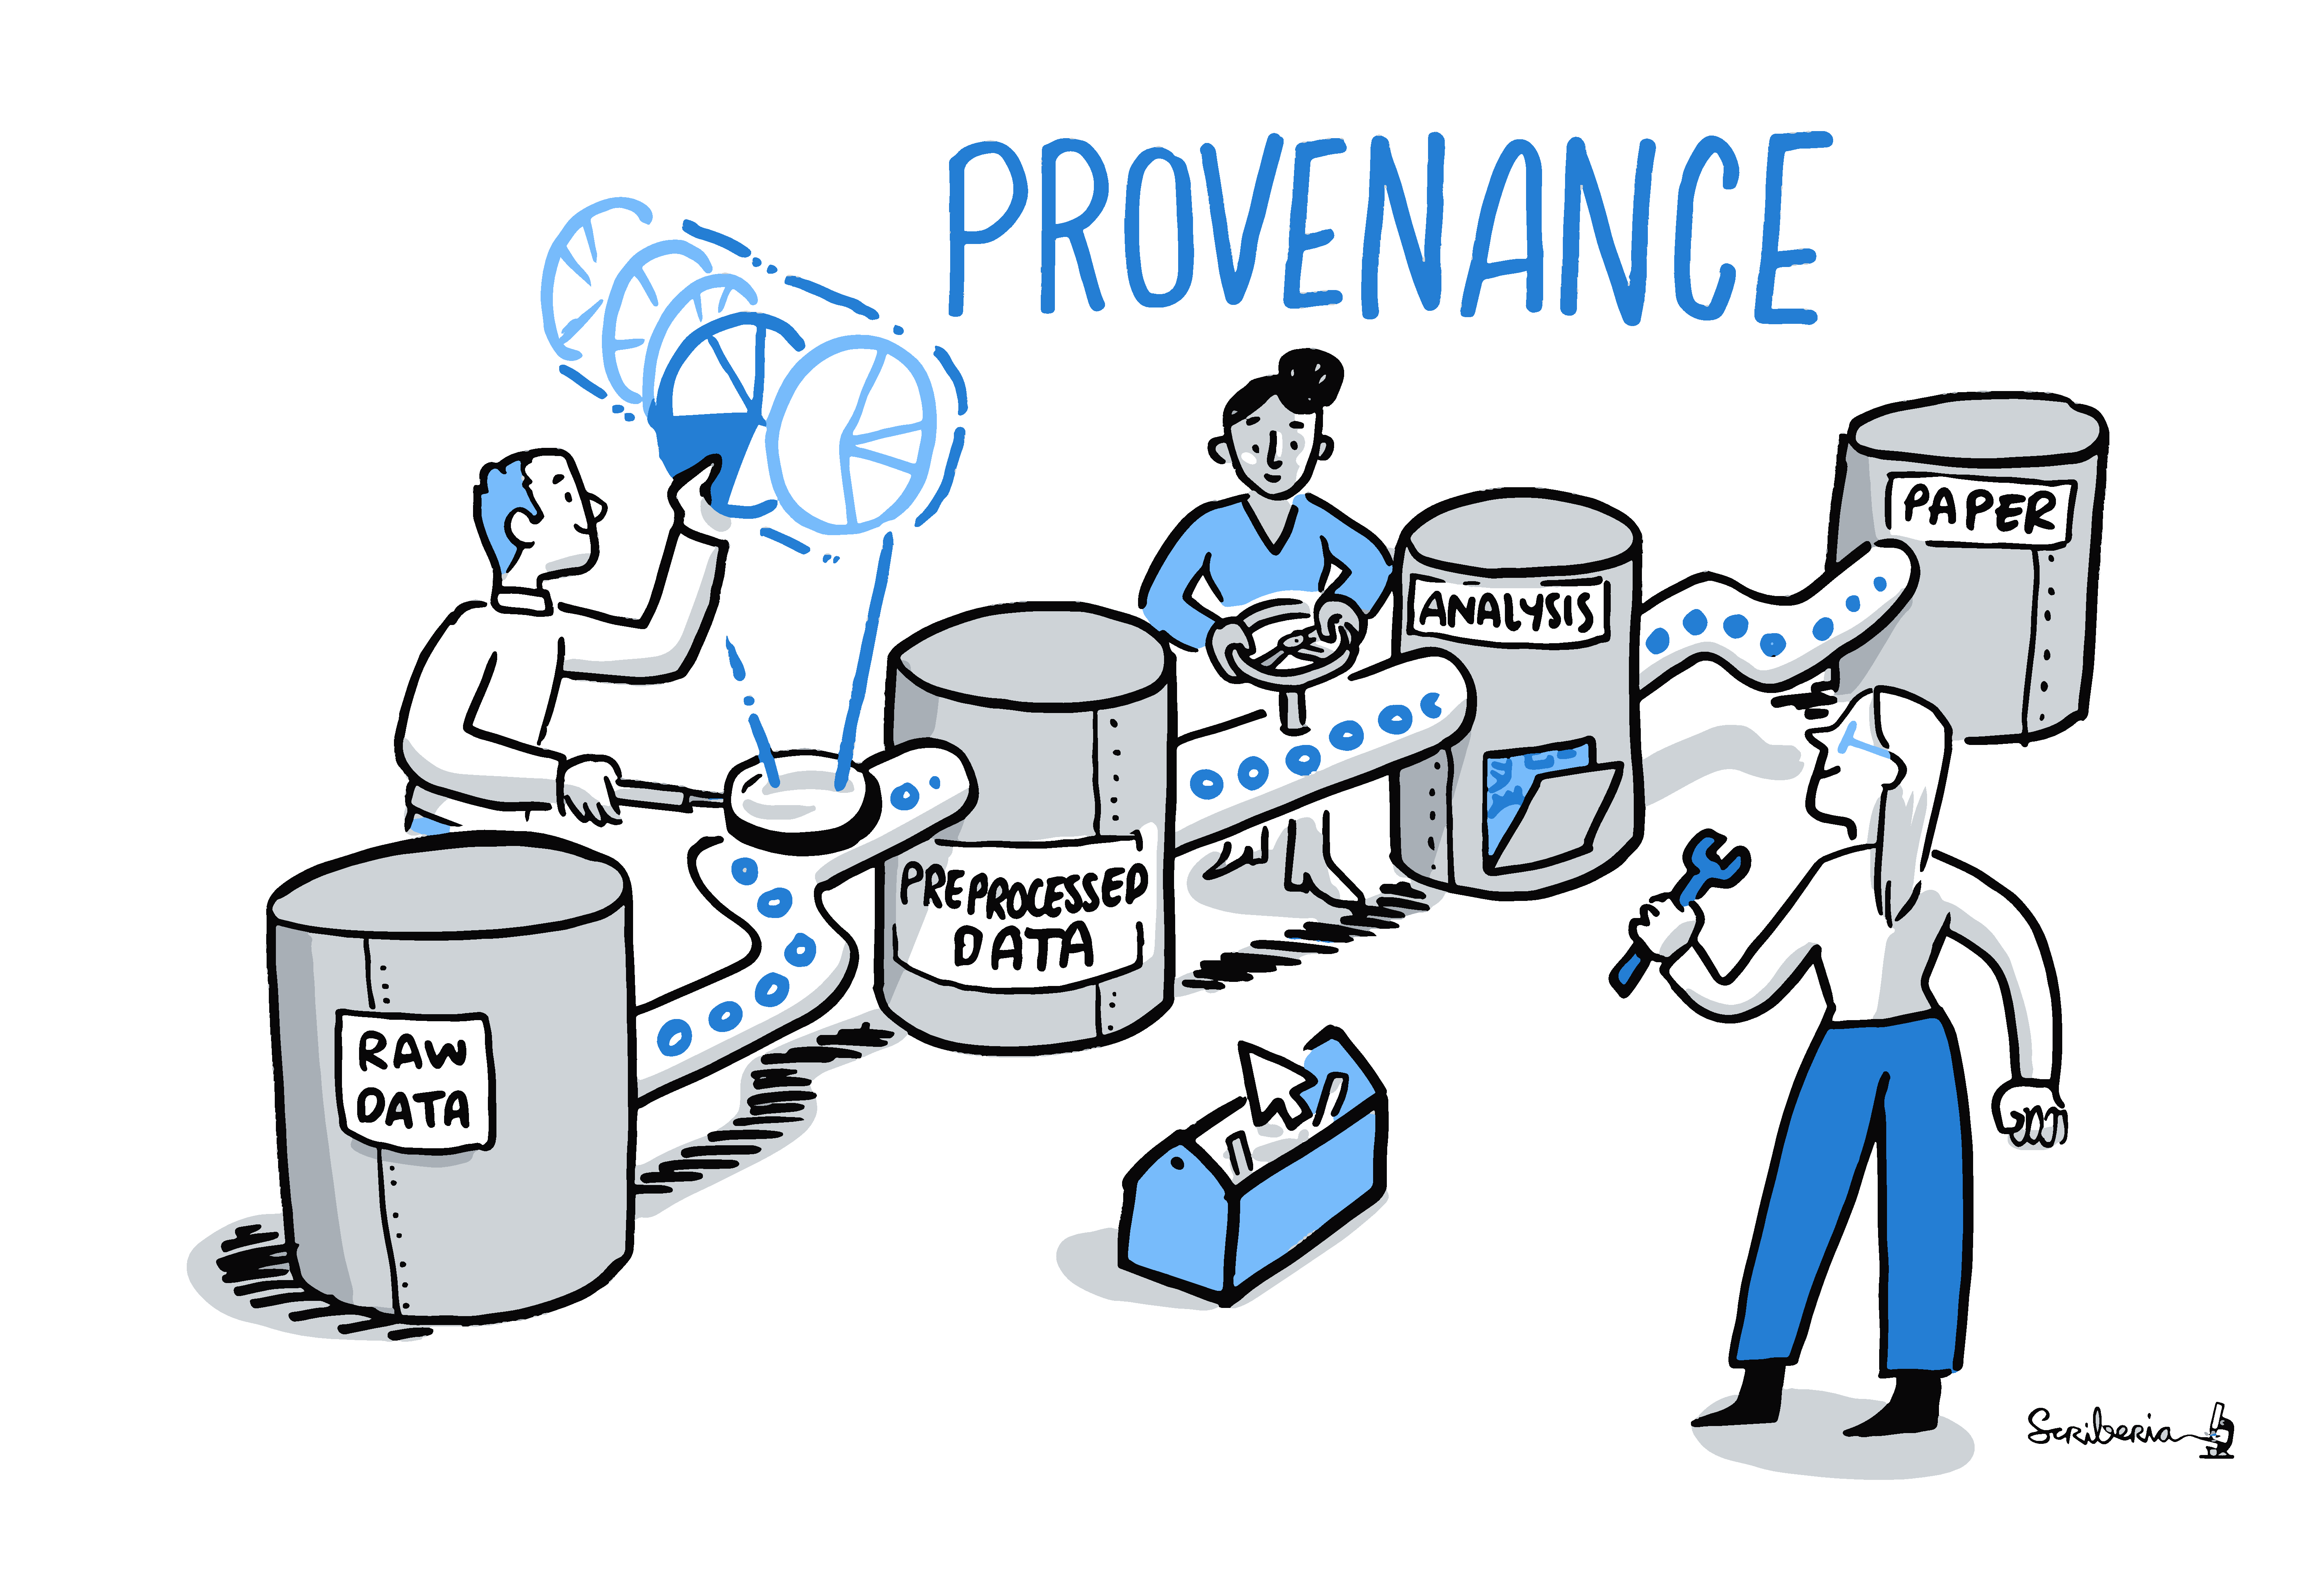
\includegraphics[width=\textwidth]{provenance.pdf}
	\caption{License: Scriberia and the Turing Way Project, CC-BY}
	\label{fig:prov1}
\end{figure}


% link to chapter 3: Research data management is a prerequisite of reproducible research

\pagebreak

\section{DataLad as a software solution for research data management challenges}

Parts of this section were published as \citet{Halchenko2021}: ``DataLad: distributed system for joint management of code, data, and their relationship'' and are appropriately marked as such.
%This introduces DataLad as a software solution for research data management

%% from datalad paper:

Code, data and computing environments are core components of scientific projects. While
the collaborative development and use of research software and code is streamlined with es-
tablished procedures and infrastructures, such as software distributions, distributed version
control systems, and social coding portals like GitHub, other components of scientific projects
are not as transparently managed or accessible. Data consumption is complicated by discon-
nected data portals that require a large variety of different data access and authentication
methods. Compared with code in software development, data tend not to be as precisely
identified because data versioning is rarely or only coarsely practiced. Scientific computation
is not reproducible enough, because data provenance, the information of how a digital file
came to be, is often incomplete and rarely automatically captured. Last but not least, in
the absence of standardized data packages, there is no uniform way to declare actionable
data dependencies and derivative relationships between inputs and outputs of a computa-
tion. DataLad aims to solve these issues by providing streamlined, transparent management
of code, data, computing environments, and their relationship. It provides targeted interfaces
and interoperability adapters to established scientific and commercial tools and services to
set up unobstructed, unified access to all elements of scientific projects. This unique set of
features enables workflows that are particularly suited for reproducible science, such as ac-
tionable process provenance capture for arbitrary command execution that affords automatic
re-execution. To this end, it builds on and extends two established tools for version control
and transport logistics, Git and git-annex.

\pagebreak

